% Options for packages loaded elsewhere
% Options for packages loaded elsewhere
\PassOptionsToPackage{unicode}{hyperref}
\PassOptionsToPackage{hyphens}{url}
\PassOptionsToPackage{dvipsnames,svgnames,x11names}{xcolor}
%
\documentclass[
  letterpaper,
  DIV=11,
  numbers=noendperiod]{scrartcl}
\usepackage{xcolor}
\usepackage{amsmath,amssymb}
\setcounter{secnumdepth}{-\maxdimen} % remove section numbering
\usepackage{iftex}
\ifPDFTeX
  \usepackage[T1]{fontenc}
  \usepackage[utf8]{inputenc}
  \usepackage{textcomp} % provide euro and other symbols
\else % if luatex or xetex
  \usepackage{unicode-math} % this also loads fontspec
  \defaultfontfeatures{Scale=MatchLowercase}
  \defaultfontfeatures[\rmfamily]{Ligatures=TeX,Scale=1}
\fi
\usepackage{lmodern}
\ifPDFTeX\else
  % xetex/luatex font selection
\fi
% Use upquote if available, for straight quotes in verbatim environments
\IfFileExists{upquote.sty}{\usepackage{upquote}}{}
\IfFileExists{microtype.sty}{% use microtype if available
  \usepackage[]{microtype}
  \UseMicrotypeSet[protrusion]{basicmath} % disable protrusion for tt fonts
}{}
\makeatletter
\@ifundefined{KOMAClassName}{% if non-KOMA class
  \IfFileExists{parskip.sty}{%
    \usepackage{parskip}
  }{% else
    \setlength{\parindent}{0pt}
    \setlength{\parskip}{6pt plus 2pt minus 1pt}}
}{% if KOMA class
  \KOMAoptions{parskip=half}}
\makeatother
% Make \paragraph and \subparagraph free-standing
\makeatletter
\ifx\paragraph\undefined\else
  \let\oldparagraph\paragraph
  \renewcommand{\paragraph}{
    \@ifstar
      \xxxParagraphStar
      \xxxParagraphNoStar
  }
  \newcommand{\xxxParagraphStar}[1]{\oldparagraph*{#1}\mbox{}}
  \newcommand{\xxxParagraphNoStar}[1]{\oldparagraph{#1}\mbox{}}
\fi
\ifx\subparagraph\undefined\else
  \let\oldsubparagraph\subparagraph
  \renewcommand{\subparagraph}{
    \@ifstar
      \xxxSubParagraphStar
      \xxxSubParagraphNoStar
  }
  \newcommand{\xxxSubParagraphStar}[1]{\oldsubparagraph*{#1}\mbox{}}
  \newcommand{\xxxSubParagraphNoStar}[1]{\oldsubparagraph{#1}\mbox{}}
\fi
\makeatother


\usepackage{longtable,booktabs,array}
\usepackage{calc} % for calculating minipage widths
% Correct order of tables after \paragraph or \subparagraph
\usepackage{etoolbox}
\makeatletter
\patchcmd\longtable{\par}{\if@noskipsec\mbox{}\fi\par}{}{}
\makeatother
% Allow footnotes in longtable head/foot
\IfFileExists{footnotehyper.sty}{\usepackage{footnotehyper}}{\usepackage{footnote}}
\makesavenoteenv{longtable}
\usepackage{graphicx}
\makeatletter
\newsavebox\pandoc@box
\newcommand*\pandocbounded[1]{% scales image to fit in text height/width
  \sbox\pandoc@box{#1}%
  \Gscale@div\@tempa{\textheight}{\dimexpr\ht\pandoc@box+\dp\pandoc@box\relax}%
  \Gscale@div\@tempb{\linewidth}{\wd\pandoc@box}%
  \ifdim\@tempb\p@<\@tempa\p@\let\@tempa\@tempb\fi% select the smaller of both
  \ifdim\@tempa\p@<\p@\scalebox{\@tempa}{\usebox\pandoc@box}%
  \else\usebox{\pandoc@box}%
  \fi%
}
% Set default figure placement to htbp
\def\fps@figure{htbp}
\makeatother





\setlength{\emergencystretch}{3em} % prevent overfull lines

\providecommand{\tightlist}{%
  \setlength{\itemsep}{0pt}\setlength{\parskip}{0pt}}



 


\KOMAoption{captions}{tableheading}
\makeatletter
\@ifpackageloaded{caption}{}{\usepackage{caption}}
\AtBeginDocument{%
\ifdefined\contentsname
  \renewcommand*\contentsname{Table of contents}
\else
  \newcommand\contentsname{Table of contents}
\fi
\ifdefined\listfigurename
  \renewcommand*\listfigurename{List of Figures}
\else
  \newcommand\listfigurename{List of Figures}
\fi
\ifdefined\listtablename
  \renewcommand*\listtablename{List of Tables}
\else
  \newcommand\listtablename{List of Tables}
\fi
\ifdefined\figurename
  \renewcommand*\figurename{Figure}
\else
  \newcommand\figurename{Figure}
\fi
\ifdefined\tablename
  \renewcommand*\tablename{Table}
\else
  \newcommand\tablename{Table}
\fi
}
\@ifpackageloaded{float}{}{\usepackage{float}}
\floatstyle{ruled}
\@ifundefined{c@chapter}{\newfloat{codelisting}{h}{lop}}{\newfloat{codelisting}{h}{lop}[chapter]}
\floatname{codelisting}{Listing}
\newcommand*\listoflistings{\listof{codelisting}{List of Listings}}
\makeatother
\makeatletter
\makeatother
\makeatletter
\@ifpackageloaded{caption}{}{\usepackage{caption}}
\@ifpackageloaded{subcaption}{}{\usepackage{subcaption}}
\makeatother
\usepackage{bookmark}
\IfFileExists{xurl.sty}{\usepackage{xurl}}{} % add URL line breaks if available
\urlstyle{same}
\hypersetup{
  pdftitle={Genetics of common complex psychiatric disorders I},
  pdfauthor={Mark James Adams},
  colorlinks=true,
  linkcolor={blue},
  filecolor={Maroon},
  citecolor={Blue},
  urlcolor={Blue},
  pdfcreator={LaTeX via pandoc}}


\title{Genetics of common complex psychiatric disorders I}
\author{Mark James Adams}
\date{}
\begin{document}
\maketitle


\section{Part 1: Biometrics}\label{part-1-biometrics}

Mark James Adams\\
Division of Psychiatry\\
\texttt{mark.adams@ed.ac.uk}\strut \\
\emph{Genetics and Environmental Influences on Behaviour and Mental
Health}

\section{\texorpdfstring{What is a \emph{``common''}, \emph{``complex''}
psychiatric
disorder?}{What is a ``common'', ``complex'' psychiatric disorder?}}\label{what-is-a-common-complex-psychiatric-disorder}

\textbf{Common:} Affects 1\% or more of the population\\
\textbf{Complex:} Inheritance cannot be explained by a single gene

Psychiatric disorders are defined by disruption to higher-order brain
functions of moods, perceptions, thoughts, beliefs, and behaviours but
usually in the absence of major neurological impairments (consciousness,
senses, memory). Psychiatric disorders include depressive and anxiety
disorders (major depressive disorder, panic disorder), manic and
psychotic disorders (bipolar disorder, schizophrenia),
obsessive-compulsive disorders, eating disorders (anorexia nervosa,
bulimia nervosa), substance-use disorders and personality disorders.
Childhood conditions like attention-deficit/hyperactivity and autism can
also be included, but only when they lead to clinically-salient
impairment or distress. There are also many shades of sadness,
hallucinations, eccentricities, mood swings, body-image preoccupations,
recreational substances use, personalities, etc that are not psychiatric
disorders but may still be informative to study from an aetiological and
genetic standpoint.

\begin{itemize}
\tightlist
\item
  Sullivan PF and Geschwind DH (2019)
  \href{https://doi.org/10.1016/j.cell.2019.01.015}{Defining the
  Genetic, Genomic, Cellular, and Diagnostic Architectures of
  Psychiatric Disorders}. \emph{Cell} doi:10.1016/j.cell.2019.01.015
\end{itemize}

\subsection{Psychiatric diagnoses}\label{psychiatric-diagnoses}

\begin{itemize}
\tightlist
\item
  Depressive disorder: Marked and persistent low mood and inability to
  feel pleasure.
\item
  Anxiety disorder: Extensive, pervasive, unrealistic, and disabling
  worry.
\item
  Bipolar disorder: Intense mood swings between mania and depression.
\item
  Schizophrenia: Peristent hallucinations and delusions that severely
  impair functioning, highly disorganised thought and speech.
\item
  Eating disorders: self-starvation or excessive over-eating,
  debilitating preoccupation with body image.
\item
  Attention-deficit/hyperactivity disorder: Early onset, developmentally
  inappropriate and persistant hyperactivity and inattention.
\item
  Autism spectrum disorders: Markedly impaired interpersonal
  interactions, non-goal-directed behaviours, and language development.
\end{itemize}

\begin{itemize}
\tightlist
\item
  Sullivan, P. F., Daly, M. J. \& O'Donovan, M. Genetic architectures of
  psychiatric disorders: the emerging picture and its implications. Nat
  Rev Genet 13, 537 551 (2012).
\item
  Frances, A. Essentials of Psychiatric Diagnosis. Guilford Press
  (2013).
\end{itemize}

\subsection{Prevalences}\label{prevalences}

\begin{itemize}
\tightlist
\item
  Depression: 3\% in a week
\item
  Schizophrenia: 1\% in lifetime
\item
  Bipolar disorder: 2\% in lifetime
\item
  Anxiety disorder: 6\% in a week
\end{itemize}

Psychiatric disorders have many causes, correlates, and consequences
(genetics, environment, family life, substance use, relationships)

Incidence of psychiatric disorders range from the common (depression,
anxiety) to the rare (bipolar disorder, schizophrenia).

\section{Why genetics?}\label{why-genetics}

Why use genetics to study mental health and psychiatric disorders?

\begin{itemize}
\tightlist
\item
  Biological understanding of genes, pathways
\item
  Shared aetiology with other disorders
\item
  Risk prediction
\item
  Drug retargeting
\item
  Causal analysis of environmental risk factors
\end{itemize}

\subsection{Genetics of categorical
traits}\label{genetics-of-categorical-traits}

\begin{figure}[H]

{\centering \pandocbounded{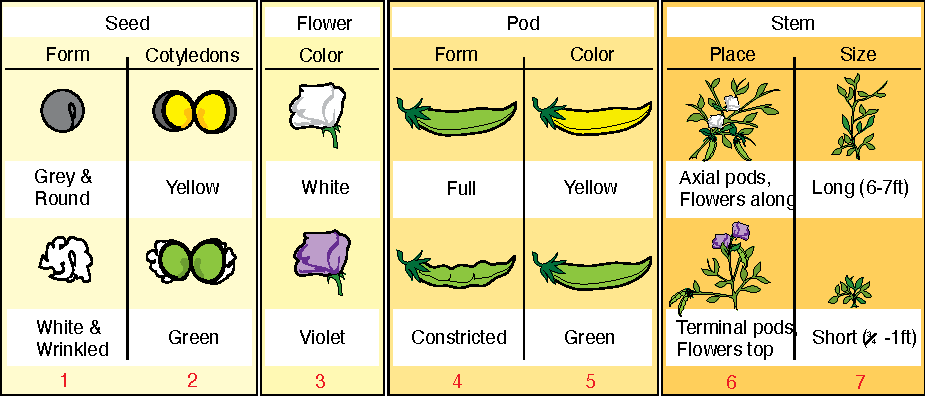
\includegraphics[keepaspectratio]{geibmh-psychgen-1_files/mediabag/assets/Mendel_seven_characters.pdf}}

}

\caption{Diagram showing the seven ``characters'' observed by Mendel}

\end{figure}%

Gregor Mendel (1822--1884), working in what is now Czechia, discovered
the transmission of traits from parents to offspring could be explained
by the inheritance of two ``elements'', which we now call alleles.
Mendel was concerned with discrete or categorical phenotypes.

\href{https://commons.wikimedia.org/wiki/File:Mendel_seven_characters.svg}{Mendel
pea plant figure} by Mariana Ruiz (LadyofHats) {[}public domain{]}

\subsection{Genetics of continuous
traits}\label{genetics-of-continuous-traits}

\pandocbounded{\includegraphics[keepaspectratio]{assets/Galton-Regression-PlateIX.png}}

Separately, Francis Galton (1822--1911), was studying the inheritance of
continuous or metric phenotypes. He noticed the parents who were tall
tended to have children that were slightly shorter than themselves (and
vice versa). This was termed ``regression to the mean'' from which the
name of the statistical method ``regression'' is derived.

\begin{quote}
``In their search for universal hereditary laws, Galton and Pearson were
driven by the linear model and the normal distribution because the
associated parameters had scientific meaning for them that went beyond
mere description.'' - Wachsmuth, A., Wilkinson, L., \& Dallal, G. E.
(2003). \href{https://dx.doi.org/10.1198/0003130031874}{Galton's Bend}.
The American Statistician, 57(3), 190--192. doi:10.1198/0003130031874
\end{quote}

For more on Galton's legacy, see
\url{https://adelphigenetics.org/history/}

\subsection{Reconciling categorical + continuous genetics = quantitative
genetics}\label{reconciling-categorical-continuous-genetics-quantitative-genetics}

\pandocbounded{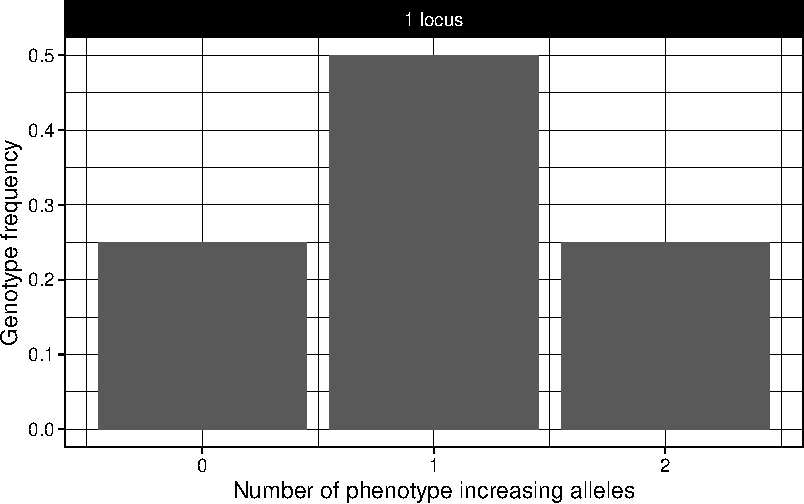
\includegraphics[keepaspectratio]{geibmh-psychgen-1_files/figure-pdf/polygenic_quantitative-1.pdf}}

Ronald Fisher reconciled the inheritance of continuous and categorical
phenotypes by showing that a continuous phenotype could be made from the
inheritance of a large number (dozens, hundreds, or thousands)
categorical genes. The term ``variance'' comes from Fisher's
discoveries.

\begin{itemize}
\tightlist
\item
  Fisher, R. A. (1918).
  \href{https://dx.doi.org/10.1017/S0080456800012163}{XV.---The
  correlation between relatives on the supposition of Mendelian
  inheritance}. \emph{Transactions of the Royal Society of Edinburgh}.
  doi:10.1017/S0080456800012163
\item
  Charlesworth and Edwards (2018).
  \href{https://doi.org/10.1111/j.1740-9713.2018.01170.x}{A century of
  variance}. \emph{Significance} 15(4).
  doi:10.1111/j.1740-9713.2018.01170.x
\item
  Bodmer et al (2021)
  \href{https://dx.doi.org/10.1038/s41437-020-00394-6}{The outstanding
  scientist, R.A. Fisher: his views on eugenics and race}.
  \emph{Heredity} doi:10.1038/s41437-020-00394-6
\end{itemize}

\subsection{Single locus with additive
effect}\label{single-locus-with-additive-effect}

Single locus with two alleles, \(\mathrm{A}_1\) and \(\mathrm{A}_2\),
and four genotypes with values:

\begin{itemize}
\tightlist
\item
  \(\mathrm{A}_1\mathrm{A}_1\): \(2a\)
\item
  \(\mathrm{A}_1\mathrm{A}_2\) and \(\mathrm{A}_2\mathrm{A}_1\): \(a\)
\item
  \(\mathrm{A}_2\mathrm{A}_2\): \(0\)
\end{itemize}

At this locus the \(\mathrm{A}_2\mathrm{A}_2\) homozygote is set as the
baseline

\subsection{}\label{section}

If allele \(\mathrm{A}_1\) has a frequency of \(p\) and \(\mathrm{A}_2\)
has frequency \(1-p\), then the genotype frequencies are:

\begin{itemize}
\tightlist
\item
  \(\mathrm{A}_1\mathrm{A}_1\): \(p^2\)
\item
  \(\mathrm{A}_1\mathrm{A}_2\) and \(\mathrm{A}_2\mathrm{A}_1\):
  \(2p(1-p)\)
\item
  \(\mathrm{A}_2\mathrm{A}_2\): \((1-p^2)\)
\end{itemize}

\subsection{}\label{section-1}

\begin{longtable}[]{@{}
  >{\raggedright\arraybackslash}p{(\linewidth - 6\tabcolsep) * \real{0.4154}}
  >{\raggedleft\arraybackslash}p{(\linewidth - 6\tabcolsep) * \real{0.1692}}
  >{\raggedleft\arraybackslash}p{(\linewidth - 6\tabcolsep) * \real{0.1077}}
  >{\raggedleft\arraybackslash}p{(\linewidth - 6\tabcolsep) * \real{0.3077}}@{}}
\toprule\noalign{}
\begin{minipage}[b]{\linewidth}\raggedright
Genotype
\end{minipage} & \begin{minipage}[b]{\linewidth}\raggedleft
Frequency
\end{minipage} & \begin{minipage}[b]{\linewidth}\raggedleft
Value
\end{minipage} & \begin{minipage}[b]{\linewidth}\raggedleft
Freq. \(\times\) Val.
\end{minipage} \\
\midrule\noalign{}
\endhead
\bottomrule\noalign{}
\endlastfoot
\(\mathrm{A}_1\mathrm{A}_1\) & \(p^2\) & \(2a\) & \(2p^2a\) \\
\(\mathrm{A}_1\mathrm{A}_2\) & \(p(1-p)\) & \(a\) & \(p(1-p)a\) \\
\(\mathrm{A}_2\mathrm{A}_1\) & \(p(1-p)\) & \(a\) & \(p(1-p)a\) \\
\(\mathrm{A}_2\mathrm{A}_2\) & \((1-p)^2\) & \(0\) & \(0\) \\
& & Mean = & \(2pa\) \\
& & Variance = & \(2p(1-p)a^2\) \\
\end{longtable}

Table based on Table 7.1, Falconer and Mackay.

\subsection{Genetic values}\label{genetic-values}

Each individual \(i\) has a genetic value at locus \(j\):

\[
g_{ij} \in [0, a_j, 2a_j]
\]

Total genetic value from \(M\) loci:

\[
G_i = \sum_{j = 1}^M g_{ij}
\]

\[
\mathrm{var}(G) = \sum_{j = 1}^M 2p_j(1-p_j)a_j^2
\]

\subsection{Polygenic traits are quantitative
traits}\label{polygenic-traits-are-quantitative-traits}

Adding up effects from a large number of genetic loci makes a continuous
phenotype.

\pandocbounded{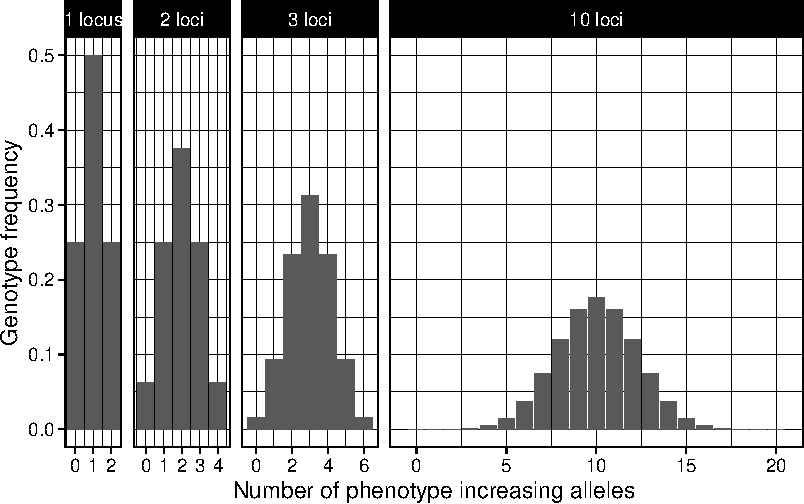
\includegraphics[keepaspectratio]{geibmh-psychgen-1_files/figure-pdf/polygenic_quantitative_10-1.pdf}}

\begin{quote}
``R. A. Fisher's 1918 paper, `The correlation between relatives on the
supposition of Mendelian inheritance', resolved the often bitter
conflict between biometricians and Mendelians, which raged for a decade
following the rediscovery of Mendel's work. Fisher showed that a complex
quantitative trait could be explained by Mendelian inheritance if
several genes affect the trait.'' - Plomin, R., Haworth, C. \& Davis, O.
\href{https://dx.doi.org/10.1038/nrg2670}{Common disorders are
quantitative traits}. \emph{Nat Rev Genet} \textbf{10}, 872-878 (2009).
doi:10.1038/nrg2670
\end{quote}

\section{Biometrics}\label{biometrics}

\subsection{What are the sources of family resemblance? How do we
quantify them
numerically?}\label{what-are-the-sources-of-family-resemblance-how-do-we-quantify-them-numerically}

\subsection{Heritability}\label{heritability}

Proportion of similarity in phenotypes that can be attributed to
similarity in genotypes.

\textbf{Model:} Phenotype (P) = Genotype (G) + Environment (E)\\
\textbf{Variance decomposition}
\[\mathrm{var}(P) = \mathrm{var}(G) + \mathrm{var}(𝐸)\]

\textbf{Proportion of variance}
\[H^2 = \frac{\mathrm{var}(G)}{\mathrm{var}(𝑃)}, e^2 = \frac{\mathrm{var}(E)}{\mathrm{var}(𝑃)}, H^2 + e^2 = 1\]

The effect \(G\) denotes all genetic effects (\(G = A + D + I\) for
additive, dominance, and epistatic variance). In the more limited case
where it is assumed genetic effects act only additively (they don't
interact with each other), then only additive genetic variance
\(\mathrm{var}(A)\) is used with (narrow-sense) heritability defined as
\(h^2 = \frac{\mathrm{var}(A)}{\mathrm{var}(P)}\).

\begin{itemize}
\tightlist
\item
  Tenesa, A., Haley, C. \href{https://dx.doi.org/10.1038/nrg3377}{The
  heritability of human disease: estimation, uses and abuses}. \emph{Nat
  Rev Genet} \textbf{14}, 139--149 (2013). doi:10.1038/nrg3377
\item
  Visscher, P., Hill, W. \& Wray, N.
  \href{https://dx.doi.org/10.1038/nrg2322}{Heritability in the genomics
  era --- concepts and misconceptions}. \emph{Nat Rev Genet} \textbf{9},
  255--266 (2008). doi:10.1038/nrg2322
\end{itemize}

\subsection{How to estimate heritability from
data}\label{how-to-estimate-heritability-from-data}

\pandocbounded{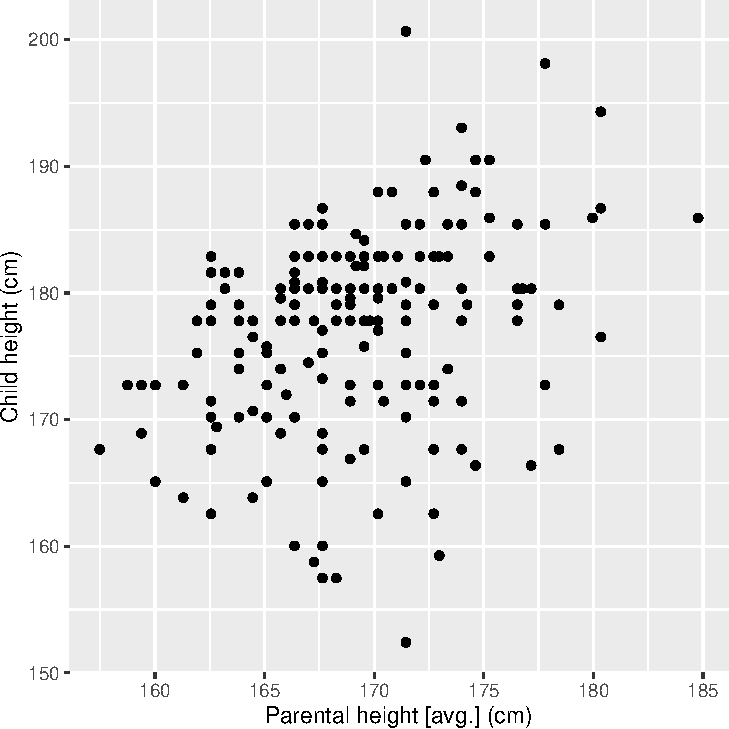
\includegraphics[keepaspectratio]{geibmh-psychgen-1_files/figure-pdf/height_parent_offspring-1.pdf}}

Plot of child (offspring) height versus the average of their parents'
heights. What is a statistic that can be used to summarise the
relationship between these two variables?

\subsection{How to estimate heritability from
data}\label{how-to-estimate-heritability-from-data-1}

\pandocbounded{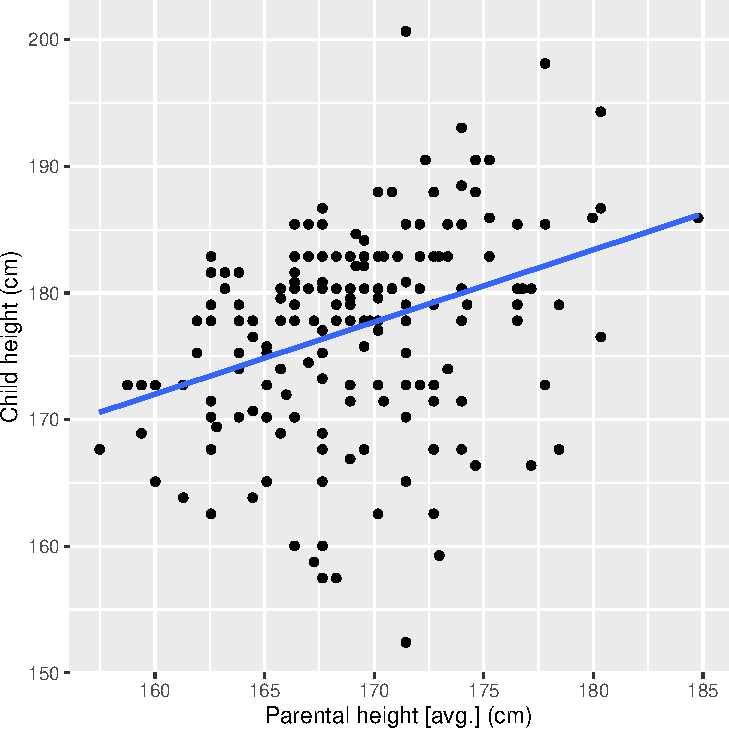
\includegraphics[keepaspectratio]{geibmh-psychgen-1_files/figure-pdf/height_parent_offspring_regress-1.pdf}}

\(\beta = \frac{\mathrm{cov}(X, Y)}{\mathrm{var}(X)}\)

Estimate the beta coefficient (slope) for a simple regression from the
covariance between predictor (\(X\)) and outcome (\(Y\)) variable
divided by the variance of the predictor (\(X\)).

\subsection{Simple model of genetic and environmental
effects}\label{simple-model-of-genetic-and-environmental-effects}

\[
P = A + E
\]

The phenotype value \(P\) is influenced by an additive genetic effect
\(A\) and and environmental effect \(E\).

For simplicity assume that \(P\) is an individual's deviation from the
average phenotype in the population.

\subsection{Simple model of genomics}\label{simple-model-of-genomics}

\[
A = a_{m_t} + a_{p_t}
\]

Each individual has two copies of the genome, one inherited from each
parent.

Here we label the genetic effect from the mother \(a_{m_t}\) (maternal)
and the genetic effect from the father \(a_{p_t}\) (paternal). These are
the transmitted genetic effects, denoted with a subscript \(t\).

\subsection{Simple model of
inheritance}\label{simple-model-of-inheritance}

\pandocbounded{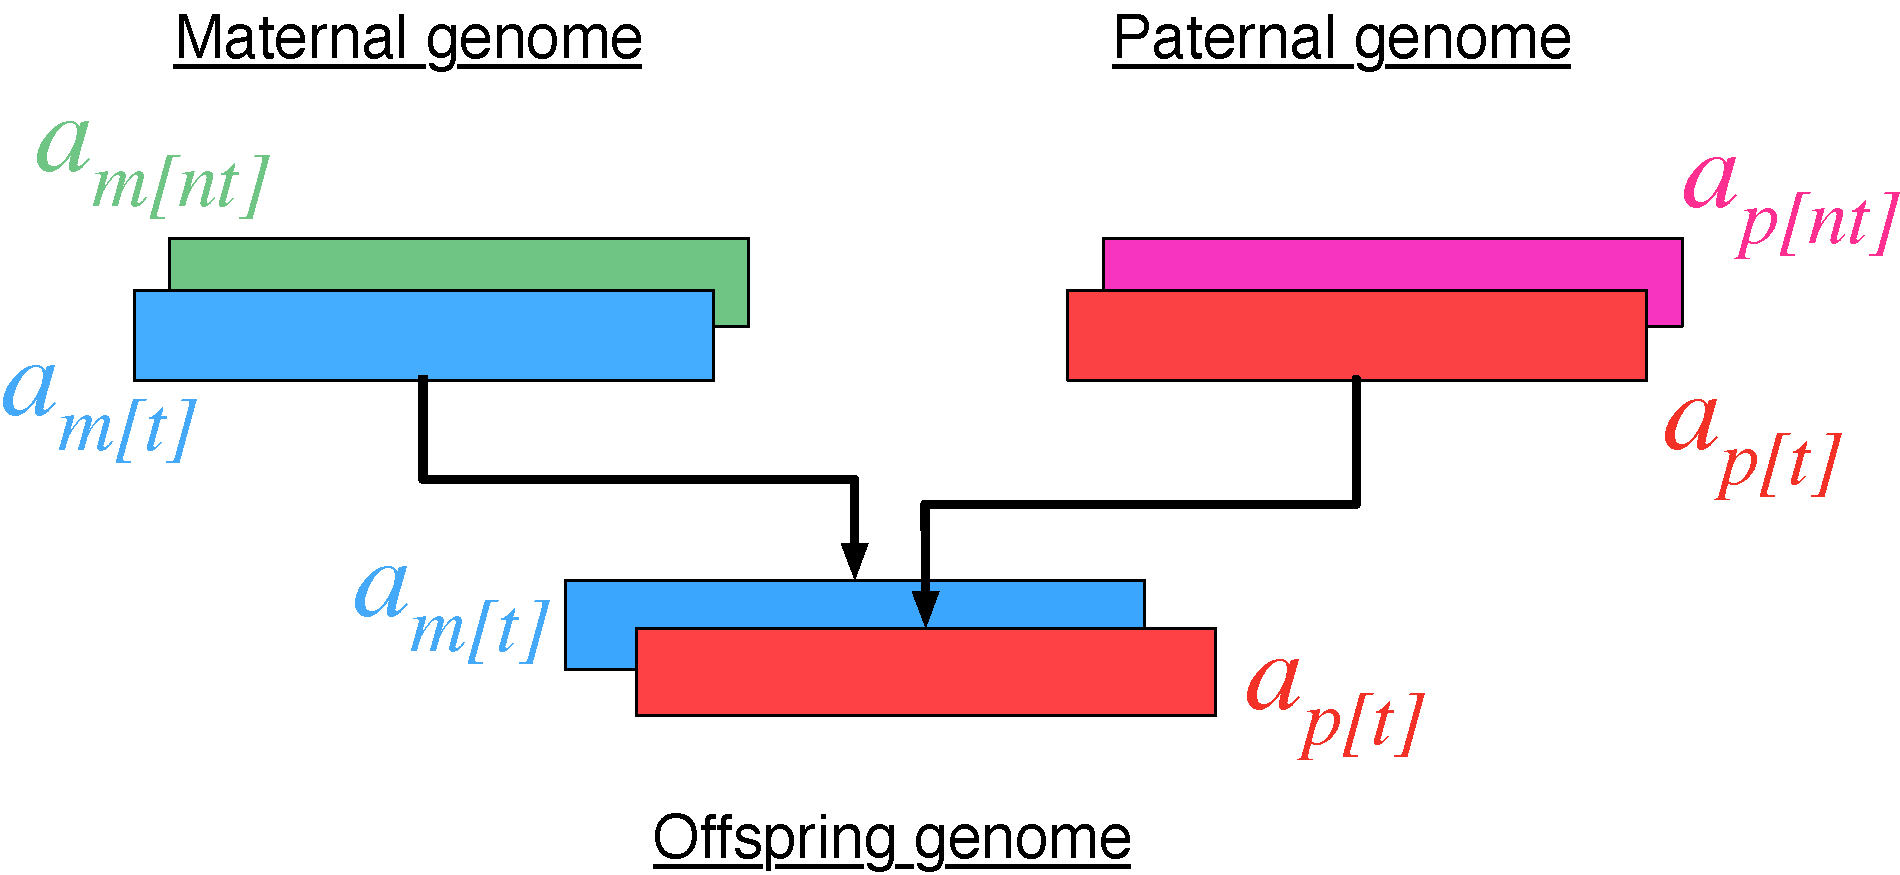
\includegraphics[keepaspectratio]{geibmh-psychgen-1_files/mediabag/assets/genetic-model.pdf}}

Each parent also has a copy of the genome which they do not pass on to
their child (``non-transmitted''), labelled \(a_{m_{nt}}\) for the
mother and \(a_{p_{nt}}\) for the father. Non-transmitted genetic
effects are written with a subscript \(nt\).

\subsection{Simple model of genetics, environment, and
inheritance}\label{simple-model-of-genetics-environment-and-inheritance}

Phenotype (\(P\)) value is the sum of the two genetic values plus an
environmental value (\(e\)).

\begin{itemize}
\tightlist
\item
  Mother's phenotype (maternal): \(P_m = a_{m_t} + a_{m_{nt}} + e_m\)
\item
  Father's phenotype (paternal): \(P_p = a_{p_t} + a_{p_{nt}}+ e_p\)
\item
  Child's phenotype (offspring): \(P_o = a_{m_t} + a_{p_t} + e_o\)
\end{itemize}

\subsection{Regression equation}\label{regression-equation}

\(\beta = \frac{\mathrm{cov}(X, Y)}{\mathrm{var}(X)}\)

\begin{itemize}
\tightlist
\item
  \(X\) = average of parents' phenotypes
\item
  \(Y\) = offspring phenotype
\end{itemize}

Therefore,
\(\beta = \frac{\mathrm{cov}(\frac{P_m + P_p}{2}, P_o)}{\mathrm{var}(\frac{P_m + P_p}{2})}\)

\subsection{Parent--offspring
covariance}\label{parentoffspring-covariance}

\[
\mathrm{cov}(\frac{P_m + P_p}{2}, P_o)
\]

The covariance term is between the average of the parental phenotypes
and the offspring phenotype.

\subsection{Simple genetic model}\label{simple-genetic-model}

\pandocbounded{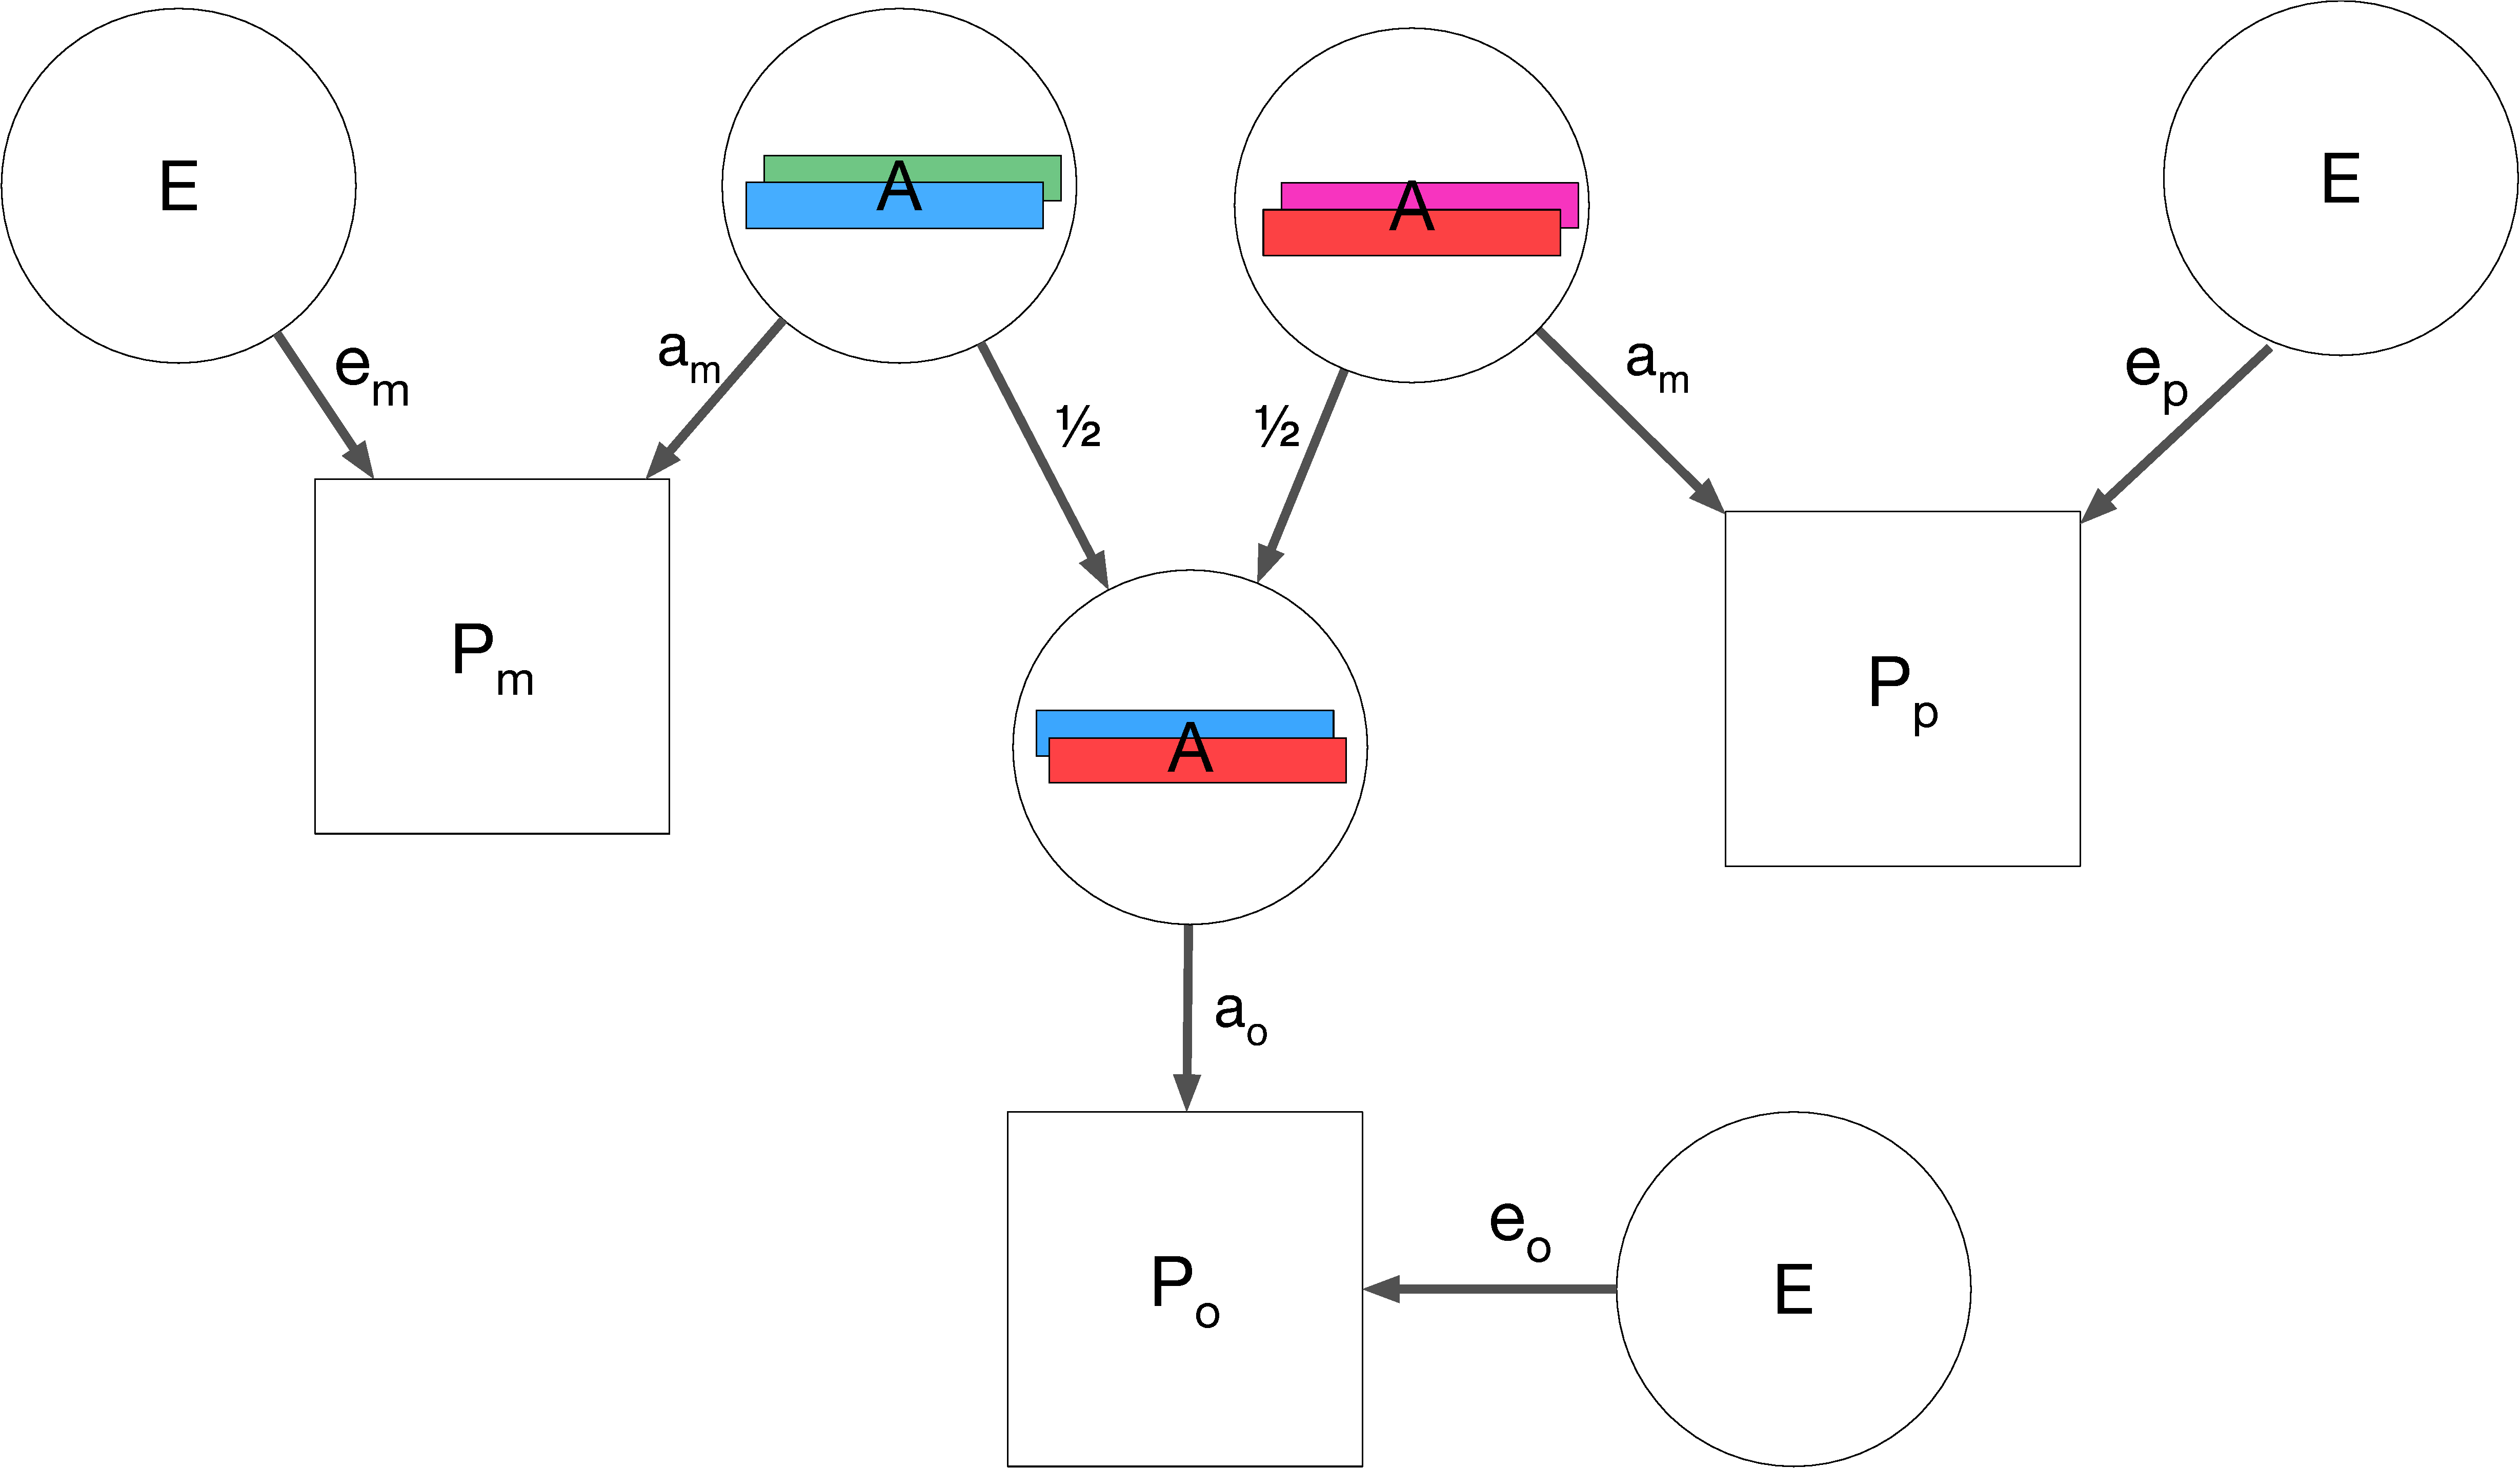
\includegraphics[keepaspectratio]{geibmh-psychgen-1_files/mediabag/assets/genetic-model-path.pdf}}

Visualisation of the simple genetic model. The observed variables
(maternal \(P_m\), paternal \(P_p\), and offspring \(P_o\) phenotypes)
are shown as squares. Unobserved (latent variables) (genetic \(A\) with
variance \(V_A\) and environment \(E\) with variance \(V_E\)). Paths are
labelled with their effects on each variable. Paths from parental to
offspring genetic variables are fixed at 0.5.

\subsection{Parent--offspring
covariance}\label{parentoffspring-covariance-1}

The only contribution to the covariance between parent and offspring
phenotypes are the transmitted parental genetic effects, which each make
up half of the genetic variance.

\[
\begin{eqnarray}
  & \mathrm{cov}(\frac{P_m + P_p}{2}, P_o) \\
= & \mathrm{cov}(\frac{P_m}{2}, P_o) + \mathrm{cov}(\frac{P_p}{2}, P_o) \\
= & \frac{1}{2} \mathrm{cov}(P_m, P_o) + \frac{1}{2} \mathrm{cov}(P_p, P_o) \\
= & \frac{1}{2} \mathrm{cov}(a_{m_t}, a_{m_t}) + \frac{1}{2} \mathrm{cov}(a_{p_t}, a_{p_t}) \\
= & \frac{1}{2} \mathrm{var}(a_{m_t}) + \frac{1}{2} \mathrm{var}(a_{p_t})\\
= & \frac{1}{2} (\frac{1}{2} V_A) + \frac{1}{2} (\frac{1}{2} V_A) \\
= & \frac{1}{2} V_A
\end{eqnarray}
\]

\subsection{Average parental variance}\label{average-parental-variance}

\[
\mathrm{var}(\frac{P_m + P_p}{2})
\]

The demoninator term is the variance of the average of the parental
phenotypes

\subsection{Average parental
variance}\label{average-parental-variance-1}

\[
\mathrm{var}(\frac{P_m + P_p}{2})
\]

The demoninator term is the variance of the average of the parental
phenotypes.

\subsection{}\label{section-2}

\[
\begin{eqnarray}
& = \mathrm{var}(\frac{P_m + P_p}{2}) \\
& = \mathrm{var}(\frac{P_m}{2}) + \mathrm{var}(\frac{P_p}{2}) \\
& = \frac{1}{4}\mathrm{var}(P_m) + \frac{1}{4} \mathrm{var}(P_p) \\
& = \frac{1}{4} V_P  + \frac{1}{4} V_P \\
& = \frac{1}{2} V_P
\end{eqnarray}
\]

The variance of the average parental phenotypes can be decomposed into
the sum of half each variance.

\subsection{Putting it all together.}\label{putting-it-all-together.}

The regression beta estimate is: \[
\beta = \frac{\mathrm{cov}(\frac{P_m + P_p}{2}, P_o)}{\mathrm{var}(\frac{P_m + P_p}{2})}
\]

Thus

\[
\beta = \frac{\frac{1}{2} V_A} {\frac{1}{2} V_P} = \frac{V_A}{V_P}  = h^2
\]

Thus heritability (\$h\^{}2) can be estimated from the regression of
offspring phentype on average parental phenotypes.

\subsection{Height data}\label{height-data}

Using the height data, we can calculate the mid-parent--offspring
covariance and mid-parent variance and then use that as an estimate for
the heritability.

\(\mathrm{cov}(\frac{P_d + P_s}{2}, P_o) =\) 12.57\\
\(\mathrm{var}(\frac{P_d + P_s}{2}) =\) 22.04\\
\(\hat{h}^2 =\) 12.57 / 22.04 = 0.57

\subsection{}\label{section-3}

Parent and offspring phenotypes become more highly correlated as
heritability increases.

\pandocbounded{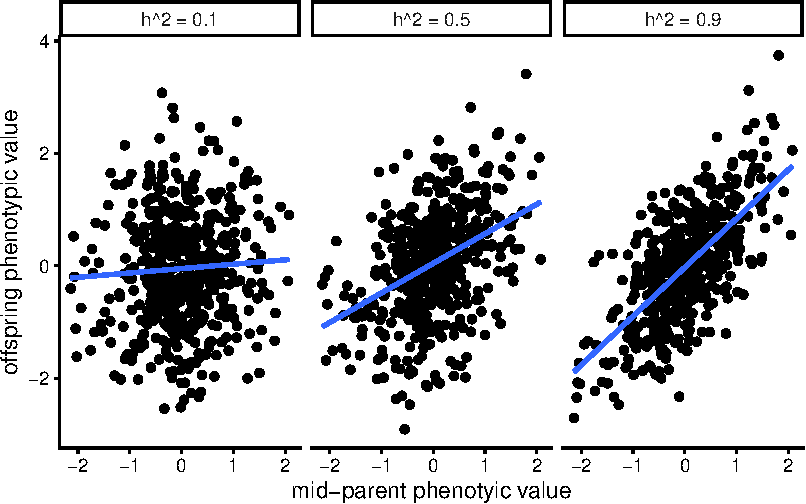
\includegraphics[keepaspectratio]{geibmh-psychgen-1_files/figure-pdf/parent_offspring_h2_sim-1.pdf}}

Wray, N. \& Visscher, P. (2008)
\href{https://www.nature.com/scitable/topicpage/estimating-trait-heritability-46889/}{Estimating
trait heritability}. Nature Education 1(1):29

\subsection{}\label{section-4}

\textbf{Mini review: What assumptions have we made when estimating
\(h^2\)?}

Parents' environments are not similar: \(\mathrm{cov}(e_d, e_s) = 0\)\\
No assortative mating: \(\mathrm{cov}(d, s) = 0\)\\
Parents do not transmit their environments:
\(\mathrm{cov}(e_o, e_d) = 0\), \(\mathrm{cov}(e_o, e_s) = 0\)\\
No gene-environment correlation: \(\mathrm{cov}(d, e_d) = 0\),
\(\mathrm{cov}(s, e_s) = 0\)\\
No genetic nature: \(\mathrm{cov}(d, e_o) = 0\),
\(\mathrm{cov}(s, e_o) = 0\)\\
No inbreeding: \(\mathrm{cov}(d, a_{m_{nt}}) = 0\),
\(\mathrm{cov}(s, a_{p_{nt}}) = 0\)\\
Genetic effects are additive: \(Y = a + a^\prime + e\)\\
Genetic influence is the same for both sexes:
\(\mathrm{var}(d + a_{m_{nt}}) =  var(s + a_{p_{nt}})\)

\subsection{Generalising to other
relatives}\label{generalising-to-other-relatives}

Heritability can also be estimated from resemblance between different
types of related pairs. The general equation is:

\[
h^2 = \frac{b}{\mathrm{r}}
\]

\(b\) = regression coefficient\\
\(\mathrm{r}\) = relatedness coefficient (``coefficient of additive
variance'')

\pandocbounded{\includegraphics[keepaspectratio]{assets/Coefficient_of_relatedness.png}}

In this notation we used normal \(\mathrm{r}\) to represent relatedness,
to disguish it from italic \(r\) for correlation coefficient.

Figure
\href{https://commons.wikimedia.org/wiki/File:Coefficient_of_relatedness.png}{Coefficient
of relatedness} CC-BY-SA Citynoise.

\subsection{Example data: depression
scores}\label{example-data-depression-scores}

Correlation of depression scores for different pairs of relatives

\pandocbounded{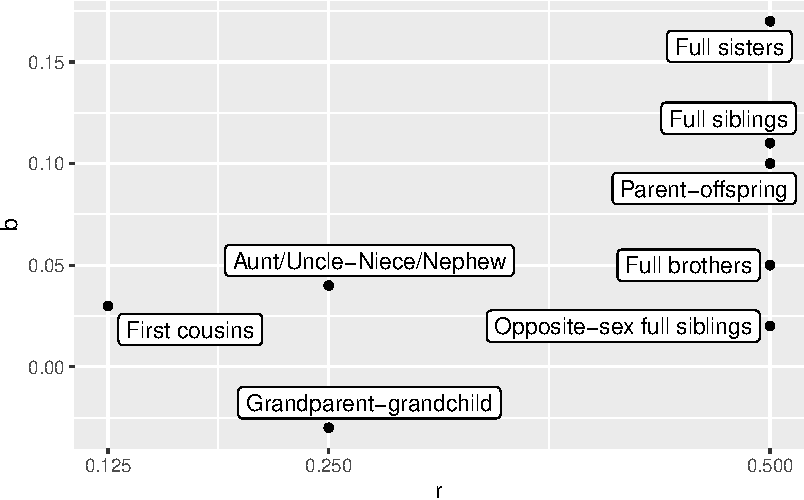
\includegraphics[keepaspectratio]{geibmh-psychgen-1_files/figure-pdf/amf_depression-1.pdf}}

Fernandez-Pujals AM et al.~(2015) Epidemiology and Heritability of Major
Depressive Disorder, Stratified by Age of Onset, Sex, and Illness Course
in Generation Scotland: Scottish Family Health Study (GS:SFHS).
\emph{PLOS ONE} 10(11): e0142197.
doi:\href{https://dx.doi.org/10.1371/journal.pone.0142197}{10.1371/journal.pone.0142197}

\subsection{Recurrance risk to
relatives}\label{recurrance-risk-to-relatives}

\[
\lambda_\mathrm{R} = \frac{P(\mathrm{affected} | \mathrm{relative\ affected})}{P(\mathrm{affected\ in\ population})} = \frac{K_\mathrm{R}}{K}
\]

\pandocbounded{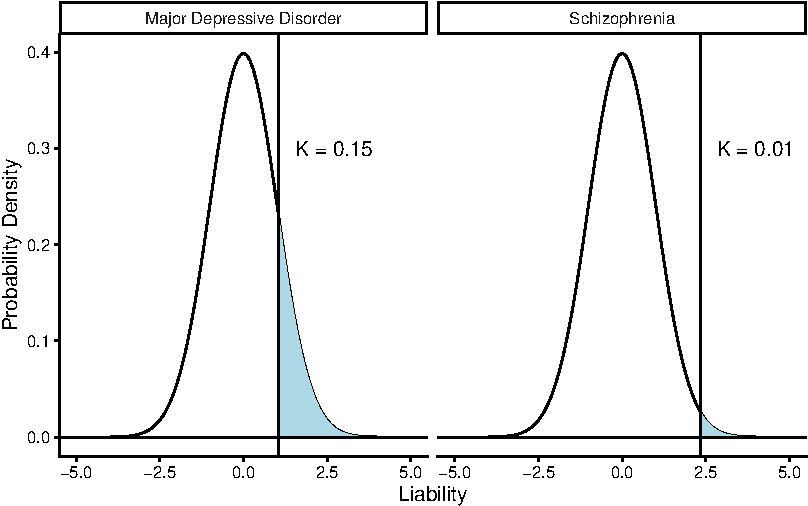
\includegraphics[keepaspectratio]{geibmh-psychgen-1_files/figure-pdf/liability_scz_mdd-1.pdf}}

Represents how much more likely a person is to be affected by a disorder
given that a relative is affected, compared to someone from the general
population.

\subsection{}\label{section-5}

Example:

\begin{itemize}
\tightlist
\item
  \(K_\mathrm{sib} = P(\mathrm{affected} | \mathrm{sibling\ affected}) = 0.09\)
\item
  \(K = P(\mathrm{affected\ in\ population}) = 0.02\)
\item
  \(\frac{K_\mathrm{sib}}{K} = \frac{0.09}{0.02} = 4.5\)
\end{itemize}

\subsection{Recurrance risk for
schizophrenia}\label{recurrance-risk-for-schizophrenia}

\pandocbounded{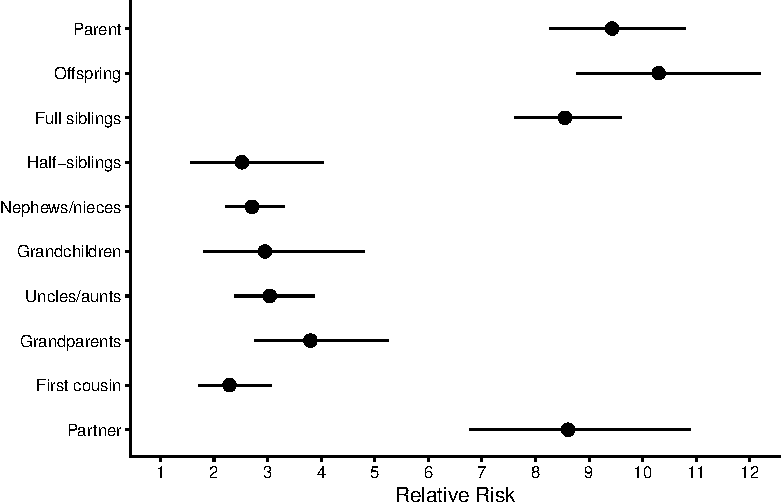
\includegraphics[keepaspectratio]{geibmh-psychgen-1_files/figure-pdf/scz_rr-1.pdf}}

Recurrance risk to relatives for schizophrenia in Sweden, which has a
baseline risk of \(K = 0.47\)\%.

Lichtenstein, P. et al.~Recurrence risks for schizophrenia in a Swedish
National Cohort. Psychol. Med. 36, 1417--1425 (2006).
doi:\href{https://dx.doi.org/10.1017/s0033291706008385}{10.1017/s0033291706008385}

\subsection{Recurrance risk and
heritability}\label{recurrance-risk-and-heritability}

\begin{itemize}
\tightlist
\item
  Score \(\mathrm{unaffected} = 0, \mathrm{affected} = 1\)
\item
  If population prevalence is \(K\), then phenotypic variance is
  \(V_\mathrm{P} = K(1-K)\) (Bernoulli distribution)
\end{itemize}

\subsection{}\label{section-6}

\begin{itemize}
\tightlist
\item
  \(Y\) = score of individual (proband)
\item
  \(Y_\mathrm{R}\) = score of relative of proband
\item
  Expectation: \(E[Y] = E[Y_\mathrm{R}] = K\)
\item
  \(K_\mathrm{R} = E[Y_\mathrm{R} | Y = 1]\)
\item
  Probability that both \(Y\) and \(Y_\mathrm{R}\) = 1:
  \(E[YY_\mathrm{R}] = K \times K_\mathrm{R}\)
\end{itemize}

\[
\mathrm{cov}(Y, Y_\mathrm{R}) = E[YY_\mathrm{R}] - E[Y] E[Y_\mathrm{R}] \\
= K \times K_\mathrm{R} - K^2 \\
\]

\begin{itemize}
\tightlist
\item
  James, J. W. Frequency in relatives for an all-or-none trait. Ann.
  Hum. Genet. 35, 47--49 (1971).
  doi:\href{https://doi.org/10.1111/j.1469-1809.1956.tb01377.x}{10.1111/j.1469-1809.1956.tb01377.x}
\item
  Risch N. Linkage strategies for genetically complex traits. I.
  Multilocus models. Am J Hum Genet. 1990 Feb;46(2):222-8. PMID: 2301392
\end{itemize}

\subsection{}\label{section-7}

\[
= K \times K_\mathrm{R} - K^2 \\
= K(K_\mathrm{R} - K) \\
= K^2 (\frac{K_\mathrm{R}}{K} - 1) \\
= K^2 (\lambda_\mathrm{R} - 1)
\]

\subsection{Heritability estimate}\label{heritability-estimate}

\[
h^2 = \frac{\mathrm{cov}_\mathrm{R}}{\mathrm{r}V_\mathrm{P}} \\
= \frac{K^2 (\lambda_\mathrm{R} - 1)}{\mathrm{r}K(1-K)} \\
= \frac{K (\lambda_\mathrm{R} - 1)}{\mathrm{r}(1-K)} \\
\]

\subsection{Recurrance risk of psychiatric
disorders}\label{recurrance-risk-of-psychiatric-disorders}

\begin{figure}[H]

{\centering \pandocbounded{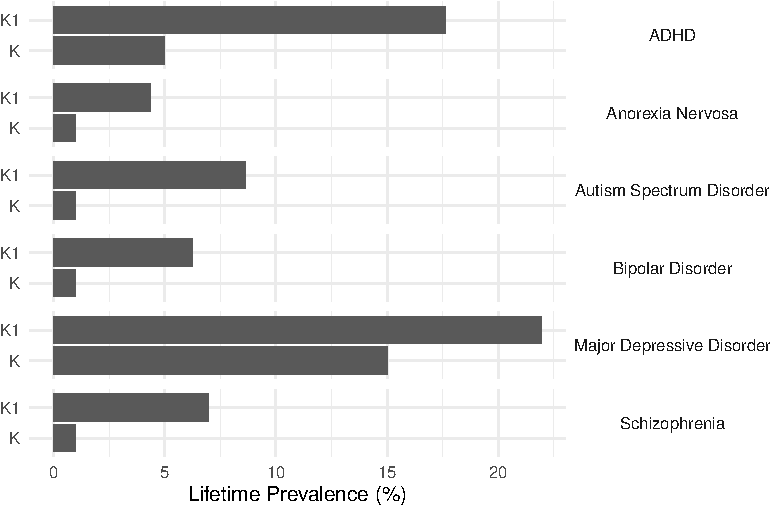
\includegraphics[keepaspectratio]{geibmh-psychgen-1_files/figure-pdf/psy_rr-1.pdf}}

}

\caption{Prevalence in population (K) and with one parent affected
(K{[}1{]})}

\end{figure}%

Baselmans, B. M. L., Yengo, L., Rheenen, W. van \& Wray, N. R. Risk in
relatives, heritability, SNP-based heritability and genetic correlations
in psychiatric disorders: a review. Biol Psychiat (2020)
doi:10.1016/j.biopsych.2020.05.034.

\subsection{Estimating environmental
effects}\label{estimating-environmental-effects}

Contrast pairs of relatives that have comparable environmental
similarity but different genetic similarity.

\pandocbounded{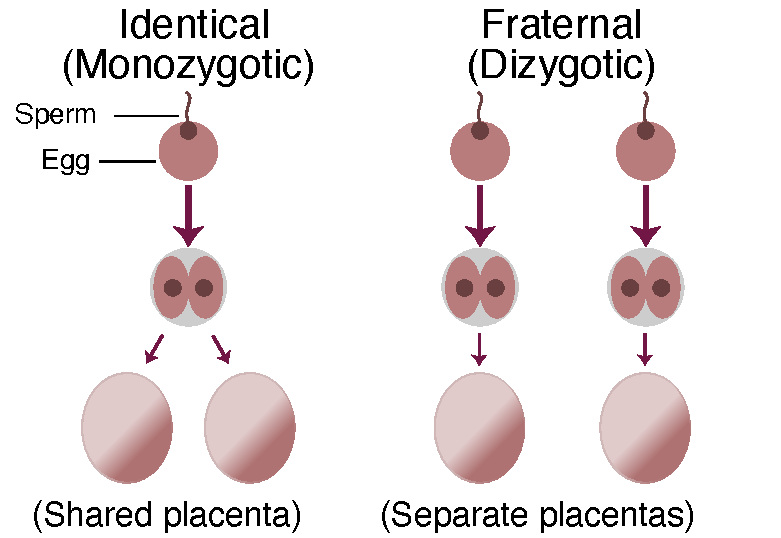
\includegraphics[keepaspectratio]{geibmh-psychgen-1_files/mediabag/assets/Identical-fraternal-sperm-egg.pdf}}

\begin{itemize}
\tightlist
\item
  Monozygotic (MZ) twins \(\mathrm{r} = 1.0\)
\item
  Dizygotic (DZ) twins \(\mathrm{r} = 0.5\)
\end{itemize}

\href{https://commons.wikimedia.org/wiki/File:Identical-fraternal-sperm-egg.svg}{Zygote
development figure} CC-BY-SA Trikly.

\subsection{Additive genetic and shared environment
effects}\label{additive-genetic-and-shared-environment-effects}

Add a shared (\(C\) or ``common'') environment to the basic genetic
model, to capture similarity between relatives attributable to
environmental factors. \(E\) represents the unique, non-shared
environment.

\[P = A + C + E\]

\[h^2 = \frac{\mathrm{var}(A)}{\mathrm{var}(P)}, c^2 = \frac{\mathrm{var}(C)}{\mathrm{var}(P)}, e^2 = \frac{\mathrm{var}(E)}{\mathrm{var}(P)}\]

\[h^2 + c^2 + e^2 = 1\]

\subsection{Twin correlations}\label{twin-correlations}

MZ twins: \(r_\mathrm{MZ} = h^2 + c^2\)

DZ twins: \(r_\mathrm{DZ} = \frac{1}{2}h^2 + c^2\)

\subsection{}\label{section-8}

\subsubsection{\texorpdfstring{Solve for genetic similarity
(\(h^2\))}{Solve for genetic similarity (h\^{}2)}}\label{solve-for-genetic-similarity-h2}

Calculate difference between MZ and DZ correlations

\[
r_\mathrm{MZ} - r_\mathrm{DZ} = (h^2 + c^2) - (\frac{1}{2}h^2 + c^2)
\]

\[
r_\mathrm{MZ} - r_\mathrm{DZ} = h^2 - \frac{1}{2}h^2 + c^2 - c^2
\]

\[
r_\mathrm{MZ} - r_\mathrm{DZ} = \frac{1}{2}h^2
\]

\[
h^2 = 2(r_\mathrm{MZ} - r_\mathrm{DZ})
\]

\subsection{}\label{section-9}

Substitute \(h^2\) into MZ equation and solve for shared environment
similarity (\(c^2\))

\[
r_\mathrm{MZ} = \underbrace{h^2} + c^2
\]

\[
r_\mathrm{MZ} = 2(r_\mathrm{MZ} - r_\mathrm{DZ}) + c^2
\]

\[
r_\mathrm{MZ} - 2(r_\mathrm{MZ} - r_\mathrm{DZ}) = c^2
\]

\[
c^2 = r_\mathrm{MZ} - 2r_\mathrm{MZ} + 2r_\mathrm{DZ}
\]

\[
c^2 = 2r_\mathrm{DZ} - r_\mathrm{MZ}
\]

\subsection{}\label{section-10}

Therefore from MZ and DZ twin correlations we can estimate:

\[
h^2 = 2(r_\mathrm{MZ} - r_\mathrm{DZ}) \\
c^2 = 2r_\mathrm{DZ} - r_\mathrm{MZ} \\
e^2 = 1 - h^2 - c^2
\]

\begin{figure}[H]

{\centering \pandocbounded{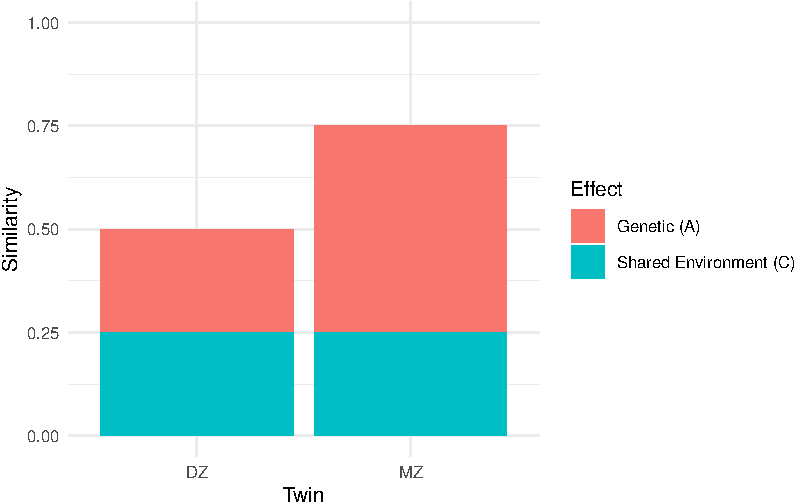
\includegraphics[keepaspectratio]{geibmh-psychgen-1_files/figure-pdf/twins_cor-1.pdf}}

}

\caption{Visualisation with \emph{r}{[}MZ{]} = 0.75 and \emph{r}{[}DZ{]}
= 0.5.}

\end{figure}%

\subsection{What do we know about psychiatric genetics from twins
studies}\label{what-do-we-know-about-psychiatric-genetics-from-twins-studies}

\pandocbounded{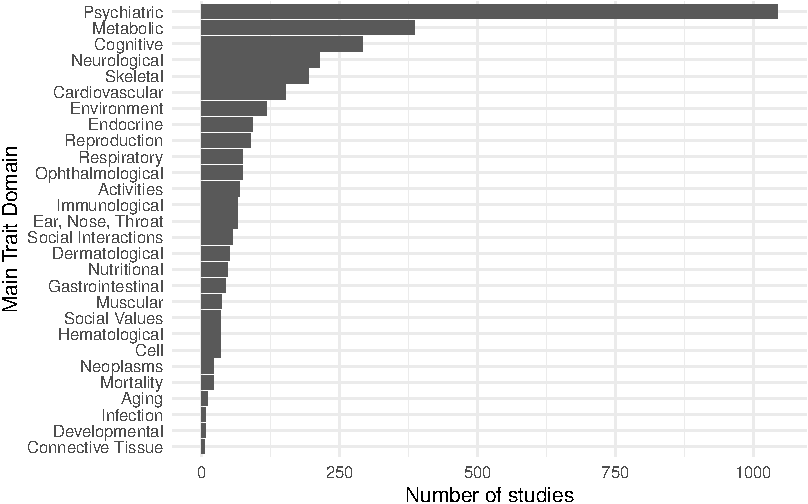
\includegraphics[keepaspectratio]{geibmh-psychgen-1_files/figure-pdf/match-class-1.pdf}}

Polderman TJC et al.~
\href{https://dx.doi.org/10.1038/ng.3285}{Meta-Analysis of the
Heritability of Human Traits based on Fifty Years of Twin Studies}
\emph{Nature Genetics} doi:10.1038/ng.3285

\subsection{Meta-analysis of twin
heritability}\label{meta-analysis-of-twin-heritability}

\begin{figure}[H]

{\centering \pandocbounded{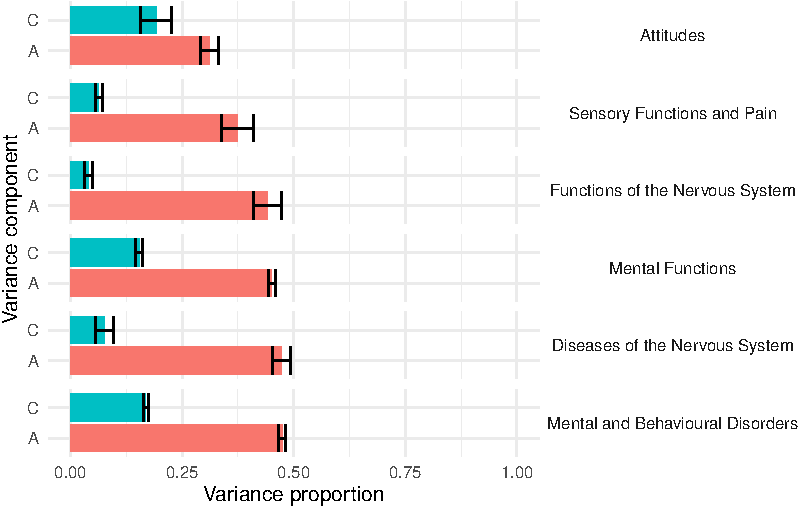
\includegraphics[keepaspectratio]{geibmh-psychgen-1_files/figure-pdf/match-meta-1.pdf}}

}

\caption{Meta-analysis of phenotype domains}

\end{figure}%

Mental and behavioural disorders are on average moderately heritable
with a smaller but substantial portion attributable to the shared
environment.

Data from \href{https://match.ctglab.nl}{\texttt{match.ctglab.nl}}.

\subsection{}\label{section-11}

\begin{figure}[H]

{\centering \pandocbounded{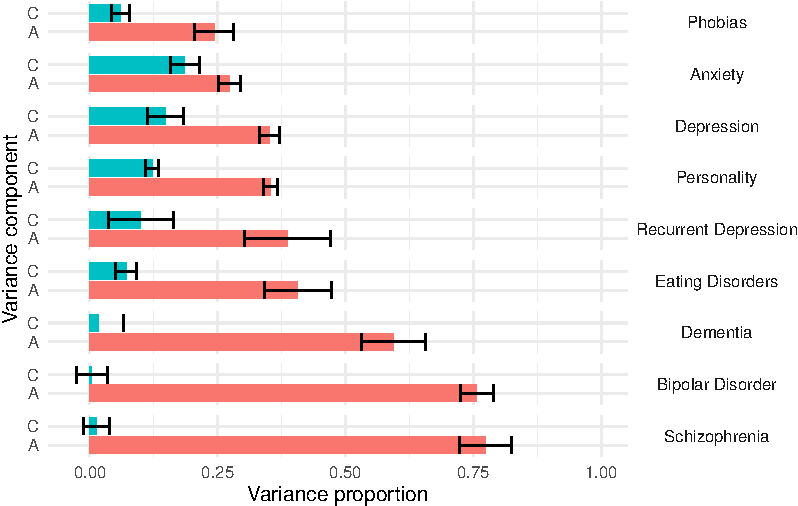
\includegraphics[keepaspectratio]{geibmh-psychgen-1_files/figure-pdf/match-meta-subchapter-1.pdf}}

}

\caption{Meta-analysis of psychiatric, neurological, and psychological
phenotypes}

\end{figure}%

\section{Genetics of depression and
schizophrenia}\label{genetics-of-depression-and-schizophrenia}

\subsection{Major depressive disorder
(MDD)}\label{major-depressive-disorder-mdd}

\begin{itemize}
\tightlist
\item
  1+ in 10 affected
\item
  7-11 years of life are lost
\item
  Global cause of ill-health
\end{itemize}

\subsection{MDD diagnostic criteria}\label{mdd-diagnostic-criteria}

1 of the 2 \textbf{cardinal} symptoms with 5 symptoms in total:

\begin{enumerate}
\def\labelenumi{\arabic{enumi}.}
\tightlist
\item
  \textbf{Low mood}
\item
  \textbf{Anhedonia}
\item
  Increase or decrease in weight or appetite
\item
  Insomnia or hypersomnia
\item
  Psychomotor agitation or slowing
\item
  Fatigue
\item
  Feelings of worthlessness/guilt
\item
  Concentration problems
\item
  Suicidal ideation
\end{enumerate}

Heterogeneous disorder: 227 possible symptom profiles.

Fried, E. I. \& Nesse, R. M. Depression is not a consistent syndrome: An
investigation of unique symptom patterns in the STAR*D study. J Affect
Disorders 172, 96--102 (2015).

\subsection{``Evidence for Multiple Genetic Factors Underlying DSM-IV
Criteria for Major
Depression''}\label{evidence-for-multiple-genetic-factors-underlying-dsm-iv-criteria-for-major-depression}

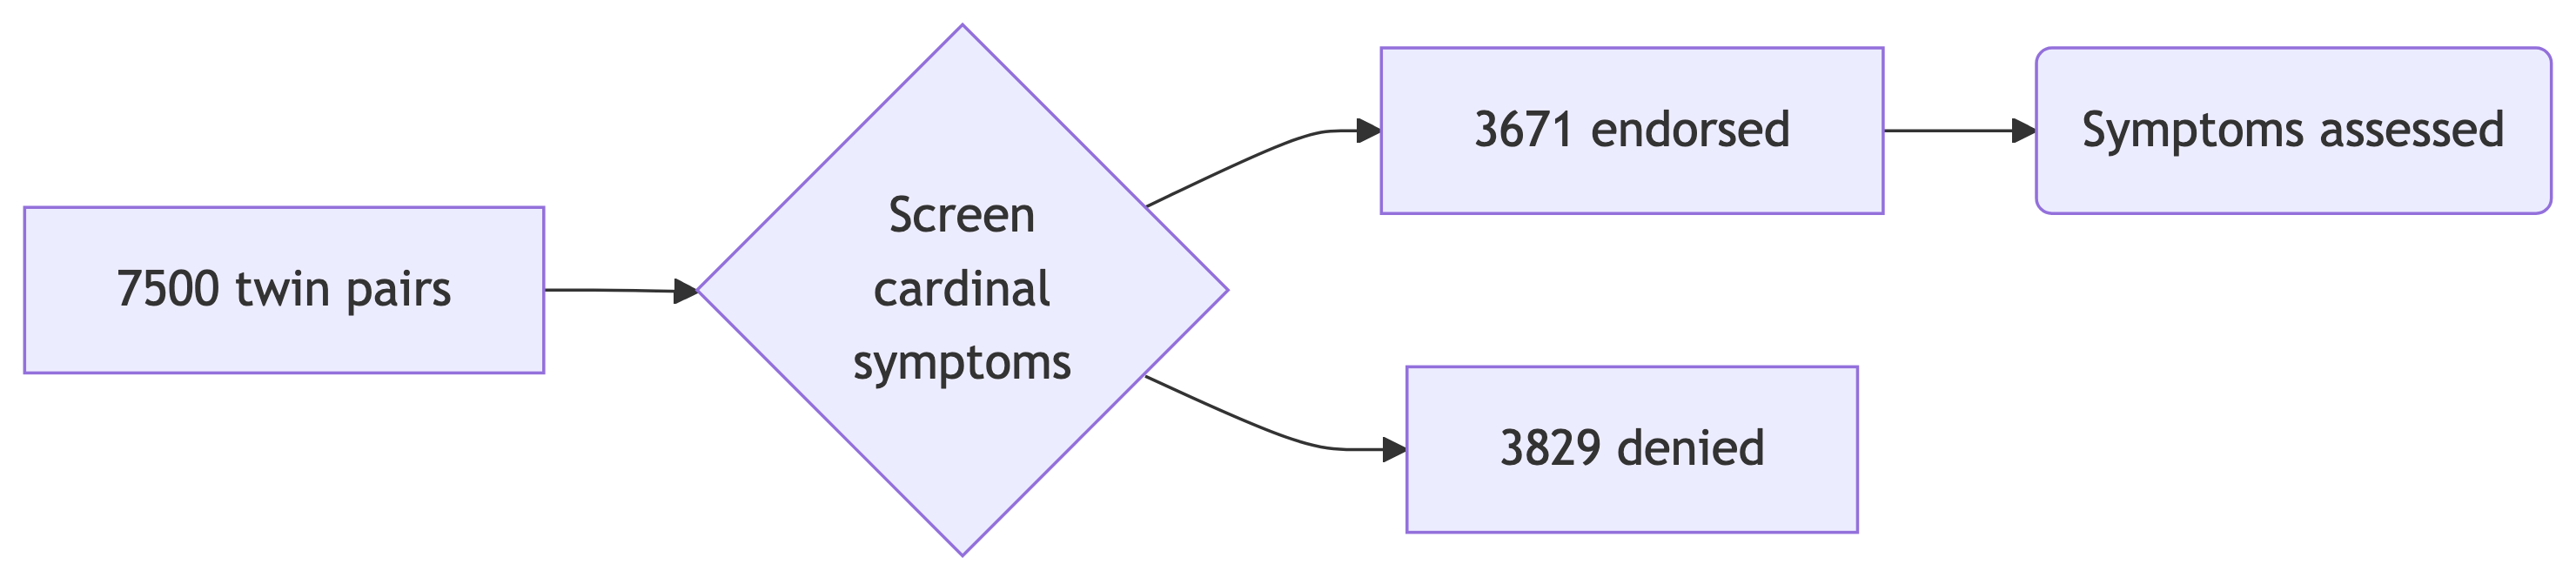
\includegraphics[width=8.75in,height=1.97in]{geibmh-psychgen-1_files/figure-latex/mermaid-figure-1.png}

Kendler, K. S., Aggen, S. H. \& Neale, M. C. Evidence for Multiple
Genetic Factors Underlying DSM-IV Criteria for Major Depression. JAMA
Psychiat 70, 599--607 (2013).

\subsection{Multivariate twin model}\label{multivariate-twin-model}

\begin{itemize}
\tightlist
\item
  analysed MZ and DZ twin cross-correlations among depression symptoms
\item
  tested 1, 2, or 3 factor models of genetic, shared environment, and
  unique environment
\end{itemize}

\subsection{Best fit model}\label{best-fit-model}

\textbf{Genetic factors}

\begin{enumerate}
\def\labelenumi{\arabic{enumi}.}
\tightlist
\item
  Psychomotor/cognitive symptoms (psychomotor, guilt, concentration,
  suicidality)
\item
  Mood symptoms (low mood, anhedonia)
\item
  Neurovegetative symptoms (weight, sleep, fatigue)
\end{enumerate}

\textbf{Individual-specific (unique) environment factors}

\begin{enumerate}
\def\labelenumi{\arabic{enumi}.}
\tightlist
\item
  General depression (low mood, anhedonia, weight, sleep, psychomotor,
  fatigue, concentration)
\item
  Mood symptoms (low mood, anhedonia, concentration)
\item
  Cognitive symptoms (guilt, suicidality)
\end{enumerate}

\subsection{External validators of genetic factor
scores}\label{external-validators-of-genetic-factor-scores}

\begin{longtable}[]{@{}lrrr@{}}
\caption{Data from Table 4 Kendler, Aggen, \& Neale. \textbf{\emph{p}
\textless{} 0.001}}\tabularnewline
\toprule\noalign{}
Validator variable & Cognitive/Motor & Core Mood & Neurovegetative \\
\midrule\noalign{}
\endfirsthead
\toprule\noalign{}
Validator variable & Cognitive/Motor & Core Mood & Neurovegetative \\
\midrule\noalign{}
\endhead
\bottomrule\noalign{}
\endlastfoot
Neuroticism & \textbf{0.54} & \textbf{0.27} & \textbf{0.30} \\
Anxiety disorder & \textbf{0.77} & \textbf{0.49} & \textbf{0.47} \\
Age at onset & \textbf{-3.00} & -1.15 & 0.37 \\
No.~of episodes & \textbf{0.55} & 0.16 & \textbf{0.23} \\
Melancholia subtype & \textbf{1.05} & \textbf{-0.43} & \textbf{1.34} \\
Unreactive mood & \textbf{0.82} & 0.10 & \textbf{0.79} \\
\end{longtable}

Cognitive/Motor factor associated with non-specific liability to
internalising disorders\\
Neurovegetative factor most strongly related to Melancholic subtype more
specific to major depression

\subsection{Schizophrenia diagnostic
criteria}\label{schizophrenia-diagnostic-criteria}

At least one \textbf{core} symptom and two or more symptoms present for
a significant period of time

\begin{enumerate}
\def\labelenumi{\arabic{enumi}.}
\tightlist
\item
  \textbf{Delusions}
\item
  \textbf{Hallucinations}
\item
  \textbf{Disorganised speech}
\item
  Grossly disorganised or catatonic behaviour
\item
  Negative symptoms
\end{enumerate}

Negative symptoms encompass deficiencies in emotional life, motivations,
thinking, and relationships

\subsection{Schizophrenia risk
factors}\label{schizophrenia-risk-factors}

\pandocbounded{\includegraphics[keepaspectratio]{assets/pmed.0020212.g001.PNG_L.png}}

Compare environmental risk factors to family history.

Figure CC-BY Sullivan PF (2005) The Genetics of Schizophrenia. PLoS Med
2(7): e212.
doi:\href{https://doi.org/10.1371/journal.pmed.0020212}{10.1371/journal.pmed.0020212}.

\section{\texorpdfstring{Why is \(h^2\) the symbol for
heritability?}{Why is h\^{}2 the symbol for heritability?}}\label{why-is-h2-the-symbol-for-heritability}

\subsection{}\label{section-12}

\pandocbounded{\includegraphics[keepaspectratio]{assets/wright-guinea-pigs-h.png}}

\(h\) for \emph{h}eritability makes sense, but why the squared term?

Sewall Wright was a geneticist who studied population and evolutionary
genetics and developed path analysis. In a path diagram of genetic,
segregation, developmental and environmental effects, the symbol \(h\)
was used as the correlation between an individual's genome and their
phenotype. If the path weights are standardised, then \(h^2\) represents
the proportion of variance in the phenotype attributable to genetics.

Wright, S. The relative importance of heredity and environment in
determining the piebald pattern of guinea-pigs. PNAS 1920.
doi:\href{https://doi.org/10.1073/pnas.6.6.320}{10.1073/pnas.6.6.320}.

\section{Coda: Longer derivation of parent-offspring covariance
(optional
material)}\label{coda-longer-derivation-of-parent-offspring-covariance-optional-material}

\subsection{Parent--offspring
covariance}\label{parentoffspring-covariance-2}

\[
\mathrm{cov}(\frac{P_m + P_p}{2}, P_o)
\]

\[
= \mathrm{cov}(\frac{a_{m_{t}} + a_{m_{nt}} + e_m + a_{p_{t}} + a_{p_{nt}}+ e_p}{2}, a_{m_{t}} + a_{p_{t}} + e_o)
\]

\subsection{Parent-offspring
covariance}\label{parent-offspring-covariance}

Expand the terms. Recall that:

\[
\mathrm{cov}(A+X,B+Y) = \\
\mathrm{cov}(A,B) + \mathrm{cov}(A,Y) + \mathrm{cov}(X,B) + \mathrm{cov}(X,Y)
\] Thus we can do a pairwise expansion to: \[
= \mathrm{cov}(\frac{a_{m_{t}}}{2} + \frac{a_{m_{nt}}}{2} + \frac{e_d}{2} + \frac{a_{p_t}}{2} + \frac{a_{p_{nt}}}{2} + \frac{e_s}{2}, a_{m_t} + a_{p_t} + e_o)
\] \[
= \mathrm{cov}(\frac{a_{m_{t}}}{2}, a_{m_{t}}) + \mathrm{cov}(\frac{a_{m_{nt}}}{2}, a_{m_{t}}) + \dotsm+ \mathrm{cov}(\frac{e_p}{2}, e_o)
\]

\subsection{Simplifications}\label{simplifications}

Some terms can be simplified.

Covariance between a genetic effect and itself \[
\mathrm{cov}(\frac{a_{m_{t}}}{2}, a_{m_{t}}), \mathrm{cov}(\frac{a_{p_{t}}}{2}}{2}, a_{p_t})
\]

Simplifies to:

\[
\mathrm{cov}(\frac{a_{m_{t}}}{2}, a_{m_{t}}) = \frac{1}{2}\mathrm{cov}(a_{m_{t}}, a_{m_{t}}) = \frac{1}{2}\mathrm{var}(a_{m_{t}})
\] \[
\mathrm{cov}(\frac{a_{p_t}}{2}, a_{p_t}) = \frac{1}{2}\mathrm{cov}(a_{p_t}, a_{p_t}) = \frac{1}{2}\mathrm{var}(a_{p_t})
\]

\subsection{Assumptions}\label{assumptions}

For some terms we might make an assumption that they are equal to 0.

\emph{Covariance between genetic effects from the same parent} \[
\mathrm{cov}(\frac{a_{m_{nt}}}{2}, a_{m_{t}}), \mathrm{cov}(\frac{a_{p_{nt}}}{2}, a_{p_t})
\]

If there is inbreeding (individual does not have ancestors that are
closely related) or assortative mating in the grandparental generation,
then genetic effects from the same parent would be expected to have a
non-zero covariance.

\emph{Covariance between genetic effects from different parents} \[
\mathrm{cov}(\frac{a_{m_{nt}}}{2}, a_{p_t}), \mathrm{cov}(\frac{a_{p_{nt}}}{2}, a_{m_{t}})
\]

If there is assortative mating between the parents, then these effects
would be expected to covary

\subsection{}\label{section-13}

\emph{Covariance between parent and offspring environment effects} \[
\mathrm{cov}(\frac{e_m}{2}, e_o), \mathrm{cov}(\frac{e_p}{2}, e_o)
\]

If aspects of the parental environment are transmitted as well or if
parents and offspring tend to encounter similar environments, then these
effects are expected to covary.

\emph{Covariance between parental genetic and offspring environmental
effects} \[
\mathrm{cov}(\frac{a_{m_{t}}}{2}, e_o), \mathrm{cov}(\frac{a_{p_t}}{2}, e_o)
\]

If parental genetic effects shape the environment of the offspring
(referred to as indirect genetic effects), then these effects are
expected to covary as well.

\subsection{}\label{section-14}

Using those assumptions the parent--offspring covariance simplifies to

\[
\mathrm{cov}(\frac{P_m + P_p}{2}, P_o) = \frac{\mathrm{var}(a_{m_{t}}) + \mathrm{var}(a_{p_t})}{2}
\]

\subsection{Parent variance}\label{parent-variance}

The denominator in the regression equation was \[
\mathrm{var}(\frac{P_m + P_p}{2})
\]

\subsection{}\label{section-15}

Using the identity \[
\mathrm{var}(aX + bY) = a^2\mathrm{var}(X) + b^2\mathrm{var}(Y) + 2ab\mathrm{cov}(X, Y)
\] the variance of the average parental phenotypes is: \[
\mathrm{var}(\frac{P_m + P_p}{2}) = \mathrm{var}(\frac{1}{2}P_m + \frac{1}{2} P_p)
\] \[
= \left(\frac{1}{2}\right)^2\mathrm{var}(P_m) + \left(\frac{1}{2}\right)^2\mathrm{var}(P_p) + 2 \cdot \frac{1}{2} \cdot \frac{1}{2} \mathrm{cov}(P_m, P_p)
\] \[
= \frac{1}{4}\mathrm{var}(P_m) + \frac{1}{4}\mathrm{var}(P_p) + \frac{1}{2} \mathrm{cov}(P_m, P_p)
\]

\subsection{}\label{section-16}

If we assume as above that there is no covariation between parental
effects (\(\mathrm{cov}(P_m, P_p) = 0\)), this simplifies to

\[
= \frac{\mathrm{var}(P_m) + \mathrm{var}(P_p)}{4}
\]

\subsection{}\label{section-17}

Thus the regression equation is:

\[
\beta = \frac{\mathrm{cov}(\frac{P_m + P_p}{2}, P_o)}{\mathrm{var}(\frac{P_m + P_p}{2})} \\
= \frac{\frac{\mathrm{var}(a_{m_{t}}) + \mathrm{var}(a_{p_t})}{2}}{\frac{\mathrm{var}(P_m) + \mathrm{var}(P_p)}{4}} \\
= 2\frac{\mathrm{var}(a_{m_{t}}) + \mathrm{var}(a_{p_t})}{\mathrm{var}(P_m) + \mathrm{var}(P_p)}
\]

\subsection{}\label{section-18}

Previously we defined

\[
A = a_{m_t} + a_{p_t}
\] thus \[
\mathrm{var}(A) = \mathrm{var}(a_{m_{t}}) + \mathrm{var}(a_{p_t})
\] and assume variances in parental phenotypes are equal \[
\mathrm{var}(P_m) = \mathrm{var}(P_s) = \mathrm{var}(P)
\]

\subsection{}\label{section-19}

Then substitute into the regression equation

\[
\beta = 2\frac{\mathrm{var}(a_{m_{t}}) + \mathrm{var}(s)}{\mathrm{var}(P_d) + \mathrm{var}(P_s)} \\
= 2 \frac{\mathrm{var}(A)}{\mathrm{var}(P) + \mathrm{var}(P)} \\
= 2 \frac{\mathrm{var}(A)}{2 \mathrm{var}(P)} \\
= \frac{\mathrm{var}(A)}{\mathrm{var}(P)} \\
= h^2
\]

In other words, the beta coefficient from the regression of offspring
phenotype on average parent phenotype yields an estimate of the
heritability!




\end{document}
